% !TeX program = xelatex
\documentclass[a4paper,10pt]{article}

% ============================================================================
% សន្លឹកកិច្ចការសិស្សបំពេញចន្លោះ ស-ខ្មៅ និងប្លង់ក្ដារខៀន/ចម្លើយគ្រូ (គ្មាន LCD / គ្មានកន្ត្រៃ)
% មេរៀនទី៣ (២.១–២.២)៖ ភាគរយ ប្រាក់ចំណេញនិងប្រាក់ខាត — ត្រូវគ្នា ១០០% នឹង LS_Plan_PCT321.tex
% ============================================================================
\usepackage[a4paper, left=1.0cm, right=1.0cm, top=0.75cm, bottom=1.00cm, footskip=0.52cm]{geometry}
\usepackage{amsmath}
\usepackage{unicode-math}
\usepackage{fontspec}
\usepackage{array, colortbl}
\usepackage[table]{xcolor}
\usepackage{enumitem}
\usepackage{pifont}
\usepackage{fancyhdr}
\usepackage{lastpage}
\usepackage{tikz}
\usepackage[most]{tcolorbox}
\usetikzlibrary{calc, arrows.meta, decorations.pathreplacing, positioning, babel}

\makeatletter
\let\@expl@@@mark@update@singlecol@structures@@\relax
\makeatother

\providecommand{\NGSFindFonts}{%
  \IfFileExists{C:/Windows/Fonts/cambria.ttc}{%
    \def\NGSSysPath{C:/Windows/Fonts/}%
    \def\NGSUserPath{C:/Users/KIT/AppData/Local/Microsoft/Windows/Fonts/}%
  }{%
    \IfFileExists{./fonts/KhmerOSsiemreap.ttf}{\def\NGSSysPath{./fonts/}\def\NGSUserPath{./fonts/}}{%
    \IfFileExists{../fonts/KhmerOSsiemreap.ttf}{\def\NGSSysPath{../fonts/}\def\NGSUserPath{../fonts/}}{%
    \IfFileExists{../../fonts/KhmerOSsiemreap.ttf}{\def\NGSSysPath{../../fonts/}\def\NGSUserPath{../../fonts/}}{%
    \IfFileExists{../../../fonts/KhmerOSsiemreap.ttf}{\def\NGSSysPath{../../../fonts/}\def\NGSUserPath{../../../fonts/}}{%
    \IfFileExists{../../../../fonts/KhmerOSsiemreap.ttf}{\def\NGSSysPath{../../../../fonts/}\def\NGSUserPath{../../../../fonts/}}{%
    \IfFileExists{../../../../../fonts/KhmerOSsiemreap.ttf}{\def\NGSSysPath{../../../../../fonts/}\def\NGSUserPath{../../../../../fonts/}}{%
    \IfFileExists{../../../../../../fonts/KhmerOSsiemreap.ttf}{\def\NGSSysPath{../../../../../../fonts/}\def\NGSUserPath{../../../../../../fonts/}}{%
      \def\NGSSysPath{../../../../../../../fonts/}\def\NGSUserPath{../../../../../../../fonts/}%
    }}}}}}}%
  }%
}
\NGSFindFonts

\setmathfont[Path={\NGSSysPath}, FontIndex=1, Scale=1.02]{cambria.ttc}
\defaultfontfeatures{Ligatures=TeX}

\setmainfont[
  Path={\NGSUserPath}, Extension=.ttf, Script=Khmer,
  BoldFont={KhmerOSsiemreap}, BoldFeatures={FakeBold=1.8},
  ItalicFont={KhmerOSsiemreap}, ItalicFeatures={FakeSlant=0.25},
  BoldItalicFont={KhmerOSsiemreap}, BoldItalicFeatures={FakeBold=1.8, FakeSlant=0.25}
]{KhmerOSsiemreap}

\newfontfamily\muol[Path={\NGSUserPath}, Extension=.ttf, Script=Khmer]{KhmerOSmuollight}
\newfontfamily\TimesEn[Path={\NGSSysPath}, Extension=.ttf, BoldFont={timesbd}, ItalicFont={timesi}, BoldItalicFont={timesbi}]{times}
\newfontfamily\CalibriFont[Path={\NGSSysPath}, Extension=.ttf]{calibri}

\XeTeXlinebreaklocale "km"
\XeTeXlinebreakskip = 0pt plus 1pt minus 0.1pt

\definecolor{panelgray}{gray}{0.94}
\definecolor{headgray}{gray}{0.85}
\definecolor{midgray}{gray}{0.76}

\pagestyle{fancy}
\fancyhf{}
\renewcommand{\headrulewidth}{0pt}
\fancyfoot[L]{\fontsize{7.4pt}{9.5pt}\selectfont អនុវិទ្យាល័យព្រះក្រសាំង \en{|} គ្រូ៖ ហុក ប៊ុនថែន \en{|} មេរៀនទី៣ (២\en{.}១--២\en{.}២) ភាគរយ ប្រាក់ចំណេញនិងប្រាក់ខាត \en{|} ថ្ងៃសុក្រ ទី២០ ខែវិច្ឆិកា ឆ្នាំ២០២៦}
\fancyfoot[R]{\fontsize{7.8pt}{9.5pt}\selectfont ទំព័រ \en{\thepage\ / \pageref{LastPage}}}

\setlength{\parindent}{0pt}
\setlength{\parskip}{0pt}
\setlength{\tabcolsep}{4pt}

\newcommand{\en}[1]{{\TimesEn #1}}
\newcommand{\enbf}[1]{{\TimesEn\bfseries #1}}
\newcommand{\unit}[1]{\,\text{\en{#1}}}
\newcommand{\riel}{\,\text{៛}}
\newcommand{\usd}{\,\text{\en{\$}}}
\newcommand{\cnum}[1]{\mbox{\fontsize{10pt}{12pt}\selectfont\ding{\numexpr181+#1\relax}}}
\newcommand{\chkbox}{\tikz[baseline=-0.15ex]\draw[black, line width=0.85pt, fill=white] (0,0) rectangle (0.24cm,0.24cm);}
\newcommand{\ansbox}[1][1.35cm]{\,\tikz[baseline=-0.65ex]\draw[black, line width=0.65pt, fill=white] (0,0) rectangle (#1, 0.42cm);\,}
\newcommand{\dotline}[1][2.2cm]{\makebox[#1]{\dotfill}}

\newcommand{\pagebanner}[2]{%
  \begin{tcolorbox}[
    enhanced, sharp corners, colback=headgray, colframe=black,
    boxrule=1.05pt, boxsep=1pt, top=2.5pt, bottom=2.5pt, left=6pt, right=6pt,
    after skip=3.5pt
  ]
    {\muol\fontsize{9.0pt}{13.2pt}\selectfont #1}\hfill{\fontsize{8.0pt}{11.2pt}\selectfont\textbf{#2}}
  \end{tcolorbox}%
}

\newcommand{\secstrip}[2]{%
  \vspace{3pt}%
  \begin{tcolorbox}[
    enhanced, sharp corners, colback=panelgray, colframe=black,
    boxrule=0.8pt, boxsep=0.8pt, top=2pt, bottom=2pt, left=5pt, right=5pt,
    after skip=3pt
  ]
    {\muol\fontsize{8.5pt}{12.2pt}\selectfont #1}\hfill{\fontsize{7.8pt}{10.8pt}\selectfont\textit{#2}}
  \end{tcolorbox}%
}

\newcolumntype{L}[1]{>{\raggedright\arraybackslash}p{#1}}
\newcolumntype{C}[1]{>{\centering\arraybackslash}p{#1}}

\begin{document}
\fontsize{9.5pt}{14.5pt}\selectfont

% ============================================================================
% ទំព័រទី ១៖ សន្លឹកកិច្ចការសិស្ស (ផ្នែកមុខ៖ E1 -> E2 -> E3)
% ============================================================================
\pagebanner{សន្លឹកកិច្ចការសិស្ស \enbf{(}២\enbf{.}១\enbf{--}២\enbf{.}២ ភាគរយ ប្រាក់ចំណេញនិងប្រាក់ខាត\enbf{)} \enbf{--} ផ្នែកមុខ}{ថ្នាក់ទី៨ \en{|} សៀវភៅគោល ទំ.៣១--៣២}

\begin{tcolorbox}[
  enhanced, sharp corners, colback=white, colframe=black,
  boxrule=0.8pt, boxsep=1.5pt, top=3.5pt, bottom=3.5pt, left=5pt, right=5pt,
  after skip=4pt
]
  \fontsize{9.0pt}{13.0pt}\selectfont
  \textbf{ឈ្មោះសិស្ស៖} \dotline[4.3cm] \quad
  \textbf{សមាជិកក្រុម៖} \dotline[4.3cm] \quad
  \textbf{ថ្នាក់ទី៖} ៨\dotline[0.9cm] \quad
  \textbf{ក្រុមទី៖} \dotline[1.0cm]
\end{tcolorbox}

% --- E1 Engage ---
\secstrip{ផ្នែកទី ១ \enbf{(E1 - Engage)} ៖ បេសកកម្មអ្នកលក់ផ្លែស្វាយនៅផ្សារកំពង់ស្វាយ}{រយៈពេល ៣ នាទី (គូស \ding{51} ក្នុង \chkbox)}

\begin{tcolorbox}[
  enhanced, sharp corners, colback=white, colframe=black,
  boxrule=0.8pt, boxsep=1.5pt, top=3.5pt, bottom=3.5pt, left=5pt, right=5pt
]
  មីងសុខាទិញផ្លែស្វាយ ១ កន្ត្រកថ្លៃដើម \textbf{$80\,000\riel$} ហើយលក់ចេញទាំងអស់បានប្រាក់ \textbf{$100\,000\riel$} (ចំណេញបាន $20\,000\riel$) ។\\[2.5pt]
  $\bullet$ \textbf{ការទស្សន៍ទាយរបស់ក្រុមអ្នក៖}\quad
  \chkbox\ \textbf{សិស្ស ក៖} ចំណេញ $\dfrac{20\,000}{100\,000}\times 100\% = \mathbf{20\%}$ \qquad
  \chkbox\ \textbf{សិស្ស ខ៖} ចំណេញ $\dfrac{20\,000}{80\,000}\times 100\% = \mathbf{25\%}$\\[2pt]
  $\bullet$ \textbf{ហេតុផលខ្លី៖} ដើម្បីគិតភាគរយប្រាក់ចំណេញ យើងត្រូវធៀបនឹង \dotline[3.4cm] (ប្រាក់លក់ / ប្រាក់ថ្លៃដើម) ។
\end{tcolorbox}

\vfill

% --- E2 Explore ---
\secstrip{ផ្នែកទី ២ \enbf{(E2 - Explore)} ៖ ច្រកឯកតា និងបន្ទះមាត្រដ្ឋានទ្វេ \enbf{100\%}}{រយៈពេល ១១ នាទី}

\textbf{សកម្មភាព ១ (\en{E2-A} — ៥ នាទី)៖ ការសរសេរបរិមាណមួយជាភាគរយនៃបរិមាណមួយទៀត (ទំ.៣១--៣២)}\\[2pt]
\begin{tcolorbox}[
  enhanced, sharp corners, colback=white, colframe=black,
  boxrule=0.8pt, boxsep=1.5pt, top=3.5pt, bottom=3.5pt, left=5pt, right=5pt
]
  \textbf{១) ឧទាហរណ៍ច្រកប្ដូរឯកតា (ទំ.៣១)៖} សរសេរ $45\unit{m}$ ជាភាគរយនៃ $1\unit{km}$ ៖\\
  \hspace*{0.3cm}$\bullet$ ប្ដូរឱ្យមានឯកតាដូចគ្នាជាមុន៖ $1\unit{km} =$ \dotline[1.6cm] $\unit{m}$ \quad $\implies$ \quad $\dfrac{45}{\dots\dots\dots}\times 100\% =$ \ansbox[1.4cm] $\%$\\[3pt]
  \textbf{២) លំហាត់គំរូបន្ទះមាត្រដ្ឋានទ្វេ (ទំ.៣២)៖} ការធ្វើតេស្តសិស្ស $40$ នាក់ ជាប់បាន $30$ នាក់ ។ ចូរបំពេញបន្ទះមាត្រដ្ឋានទ្វេខាងក្រោម៖\\[2pt]
  {\centering
  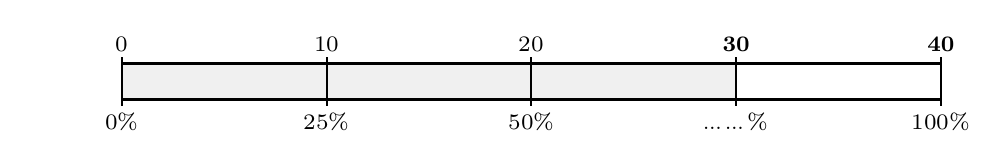
\begin{tikzpicture}[x=1cm, y=1cm, every node/.style={font=\footnotesize, text=black}]
    \fill[panelgray] (1.8,0.42) rectangle (9.6,0.88);
    \draw[black, line width=0.9pt] (1.8,0.42) rectangle (12.2,0.88);
    \foreach \x in {1.8, 4.4, 7.0, 9.6, 12.2} {
      \draw[black, line width=0.7pt] (\x,0.34) -- (\x,0.96);
    }
    \node[left=2pt] at (1.78,1.12) {\textbf{ចំនួនសិស្ស៖}};
    \node[left=2pt] at (1.78,0.14) {\textbf{ភាគរយ៖}};
    \node at (1.8,1.12) {$0$}; \node at (4.4,1.12) {$10$}; \node at (7.0,1.12) {$20$}; \node at (9.6,1.12) {$\mathbf{30}$}; \node at (12.2,1.12) {$\mathbf{40}$};
    \node at (1.8,0.14) {$0\%$}; \node at (4.4,0.14) {$25\%$}; \node at (7.0,0.14) {$50\%$}; \node at (9.6,0.14) {$\dots\dots\%$}; \node at (12.2,0.14) {$100\%$};
  \end{tikzpicture}\par}
  \vspace{2pt}
  \hspace*{0.3cm}$\implies$ ភាគរយនៃសិស្សប្រឡងជាប់គឺ $\dfrac{30}{40}\times 100\% =$ \ansbox[1.4cm] $\%$ ។
\end{tcolorbox}

\vspace{4pt}
\textbf{សកម្មភាព ២ (\en{E2-B} — ៦ នាទី)៖ ការកំណត់ប្រាក់ថ្លៃដើមស្មើ $100\%$ ក្នុងករណីចំណេញ និងខាត (ទំ.៣២)}\\[2pt]
\begin{tcolorbox}[
  enhanced, sharp corners, colback=white, colframe=black,
  boxrule=0.8pt, boxsep=1.5pt, top=3.5pt, bottom=3.5pt, left=5pt, right=5pt
]
  {\centering\renewcommand{\arraystretch}{1.24}
  \begin{tabular}{|L{4.2cm}|L{6.3cm}|L{6.5cm}|}
    \hline
    \cellcolor{headgray}\textbf{ករណីលក់ដូរ} & \cellcolor{headgray}\textbf{រូបមន្តរកប្រាក់ចំណេញ ឬ ប្រាក់ខាត} & \cellcolor{headgray}\textbf{បរិមាណគោល $100\%$ (ភាគបែង)} \\ \hline
    \textbf{១) លក់ចំណេញ} (លក់ $>$ ដើម) & ប្រាក់ចំណេញ $=$ ថ្លៃលក់ $-$ \dotline[2.2cm] & គូសរង្វង់៖ \textbf{( ប្រាក់ថ្លៃដើម \; / \; ថ្លៃលក់ )} \\ \hline
    \textbf{២) លក់ខាត} (លក់ $<$ ដើម) & ប្រាក់ខាត $=$ \dotline[2.2cm] $-$ ថ្លៃលក់ & គូសរង្វង់៖ \textbf{( ប្រាក់ថ្លៃដើម \; / \; ថ្លៃលក់ )} \\ \hline
  \end{tabular}\par}
\end{tcolorbox}

\vfill

% --- E3 Explain ---
\secstrip{ផ្នែកទី ៣ \enbf{(E3 - Explain)} ៖ សង្ខេបរូបមន្តភាគរយ និងធនាគារហេតុផល \enbf{B\&W}}{រយៈពេល ៦ នាទី}

\begin{tcolorbox}[
  enhanced, sharp corners, colback=white, colframe=black,
  boxrule=0.95pt, boxsep=1.6pt, top=3.5pt, bottom=3.5pt, left=5.5pt, right=5.5pt
]
  $\bullet$ \textbf{ជាទូទៅ ២.១ (ទំ.៣២)៖} បរិមាណ $a$ ជាភាគរយនៃ $b$ (ឯកតាដូចគ្នា) គឺ $\dfrac{a}{b}\times$ \ansbox[1.3cm] ។\\[3pt]
  $\bullet$ \textbf{រូបមន្ត ២.២ (ទំ.៣២)៖} \quad
  ភាគរយប្រាក់ចំណេញ $= \dfrac{\text{ប្រាក់ចំណេញ}}{\dots\dots\dots\dots\dots}\times 100\%$ \qquad
  ភាគរយប្រាក់ខាត $= \dfrac{\text{ប្រាក់ខាត}}{\dots\dots\dots\dots\dots}\times 100\%$\\[3pt]
  \hrule height 0.5pt
  \vspace{2.5pt}
  {\fontsize{8.7pt}{12.5pt}\selectfont
  \textbf{ធនាគារហេតុផល (\en{Warrant Bank})៖}\quad
  \cnum{1} ប្ដូរឯកតាឱ្យដូចគ្នាមុនសរសេរ $\frac{a}{b}\times 100\%$ \quad
  \cnum{2} គូសរង្វង់\textbf{ប្រាក់ថ្លៃដើម $= 100\%$} ជាភាគបែងជានិច្ច\\
  \cnum{3} ចំណេញ $=$ លក់ $-$ ដើម \en{|} ខាត $=$ ដើម $-$ លក់ \quad
  \cnum{4} ថ្លៃលក់ $=$ ថ្លៃដើម $+$ ចំណេញ (ឬ $=$ ថ្លៃដើម $-$ ខាត)}
\end{tcolorbox}

\newpage

% ============================================================================
% ទំព័រទី ២៖ សន្លឹកកិច្ចការសិស្ស (ផ្នែកខាងខ្នង៖ E4 -> E5 -> កិច្ចការផ្ទះ)
% ============================================================================
\pagebanner{សន្លឹកកិច្ចការសិស្ស \enbf{(}២\enbf{.}១\enbf{--}២\enbf{.}២ ភាគរយ ប្រាក់ចំណេញនិងប្រាក់ខាត\enbf{)} \enbf{--} ផ្នែកខាងខ្នង}{ថ្នាក់ទី៨ \en{|} សៀវភៅគោល ទំ.៣២--៣៣, ៤១--៤២}

% --- E4 Elaborate ---
\secstrip{ផ្នែកទី ៤ \enbf{(E4 - Elaborate)} ៖ លំហាត់គំរូរថយន្តលក់បន្តពីរដំណាក់កាល (ទំ.៣២--៣៣)}{រយៈពេល ១០ នាទី}

\begin{tcolorbox}[
  enhanced, sharp corners, colback=white, colframe=black,
  boxrule=0.8pt, boxsep=1.8pt, top=3.5pt, bottom=3.5pt, left=5.5pt, right=5.5pt
]
  \textbf{លំហាត់គំរូ (ទំ.៣២--៣៣)៖} ក្រុមហ៊ុននាំចូលរថយន្តមួយទិញរថយន្តថ្មីមួយគ្រឿងថ្លៃដើម $75\,000\usd$ ហើយលក់ឱ្យ\textbf{លោកលីស្រ៊ុន}ថ្លៃ $84\,000\usd$ ។ ពីរឆ្នាំក្រោយមក លោកលីស្រ៊ុនបានលក់រថយន្តនេះឱ្យ\textbf{លោកហេងលីម}ថ្លៃ $60\,000\usd$ ។\\[3pt]
  $\bullet$ \textbf{ក. រកភាគរយប្រាក់ចំណេញរបស់ក្រុមហ៊ុន៖}\\
  \hspace*{0.3cm}-- ប្រាក់ថ្លៃដើមរបស់ក្រុមហ៊ុន (\cnum{2}) $=$ \dotline[2.0cm] $\usd$ \quad;\quad ប្រាក់ចំណេញ (\cnum{3}) $= 84\,000 - 75\,000 =$ \dotline[1.8cm] $\usd$\\[2pt]
  \hspace*{0.3cm}-- ភាគរយប្រាក់ចំណេញសម្រាប់ក្រុមហ៊ុន $= \dfrac{\dots\dots\dots\dots}{75\,000}\times 100\% =$ \ansbox[1.4cm] $\%$\\[3pt]
  $\bullet$ \textbf{ខ. រកភាគរយប្រាក់ខាតរបស់លោកលីស្រ៊ុន (ប្រយ័ត្នថ្លៃដើមថ្មី \cnum{2}!)៖}\\
  \hspace*{0.3cm}-- ប្រាក់ថ្លៃដើមដែលលោកលីស្រ៊ុនចំណាយទិញ $=$ \dotline[2.0cm] $\usd$ \quad;\quad ប្រាក់ខាត $= 84\,000 - 60\,000 =$ \dotline[1.8cm] $\usd$\\[2pt]
  \hspace*{0.3cm}-- ភាគរយប្រាក់ខាតរបស់លោកលីស្រ៊ុន $= \dfrac{24\,000}{\dots\dots\dots\dots}\times 100\% \approx$ \ansbox[1.6cm] $\%$\\[3pt]
  {\fontsize{8.7pt}{12.2pt}\selectfont \textbf{ឆ្លុះបញ្ចាំង (\en{EIA Looking-Back})៖} ហេតុអ្វីក្នុងសំណួរ (ខ) យើងមិនយក $24\,000\usd$ ចែកនឹង $75\,000\usd$? ព្រោះថ្លៃដើមរបស់លោកលីស្រ៊ុនគឺ \dotline[1.8cm] $\usd$!}
\end{tcolorbox}

\vfill

% --- E5 Evaluate ---
\secstrip{ផ្នែកទី ៥ \enbf{(E5 - Evaluate)} ៖ លំហាត់ប្រតិបត្តិ សំណួរវិនិច្ឆ័យ \enbf{A--D} និងសំបុត្រចេញ}{រយៈពេល ១០ នាទី}

\noindent
\begin{minipage}[t]{9.25cm}
  \begin{tcolorbox}[
    enhanced, sharp corners, colback=white, colframe=black,
    boxrule=0.8pt, boxsep=1.5pt, top=3.5pt, bottom=3.5pt, left=4.5pt, right=4.5pt
  ]
    \textbf{១) ប្រតិបត្តិទី ១ (ទំ.៣២ — ពិន្ទុ និងប្ដូរឯកតា)៖}\\
    $\bullet$ គណិតវិទ្យាបាន $95$ ក្នុង $100$ ពិន្ទុ $=$ \dotline[1.4cm] $\%$\\[2pt]
    $\bullet$ ភាសាខ្មែរបាន $92$ ក្នុង $100$ ពិន្ទុ $=$ \dotline[1.4cm] $\%$\\[2pt]
    $\bullet$ សរសេរ $350\unit{g}$ ជាភាគរយនៃ $2\unit{kg}$ (\cnum{1})៖\\
    \hspace*{0.2cm}$2\unit{kg} =$ \dotline[1.3cm] $\unit{g} \implies \dfrac{350}{\dots\dots}\times 100\% =$ \ansbox[1.3cm] $\%$
  \end{tcolorbox}
\end{minipage}%
\hfill
\begin{minipage}[t]{9.25cm}
  \begin{tcolorbox}[
    enhanced, sharp corners, colback=white, colframe=black,
    boxrule=0.8pt, boxsep=1.5pt, top=3.5pt, bottom=3.5pt, left=4.5pt, right=4.5pt
  ]
    \textbf{២) ប្រតិបត្តិទី ២ (ទំ.៣៣ — ម៉ូតូពូសុខ) និងបិទ \en{E1}៖}\\
    ពូសុខទិញម៉ូតូថ្លៃ $2\,240\,000\riel$ លក់វិញខាតអស់ $22\%$ ៖\\[2pt]
    $\bullet$ ប្រាក់ខាត $= \frac{22}{100}\times 2\,240\,000 =$ \dotline[2.0cm] $\riel$\\[2pt]
    $\bullet$ ថ្លៃលក់ចេញ (\cnum{4}) $=$ \ansbox[2.2cm] $\riel$\\[2pt]
    $\bullet$ \textbf{បិទ \en{E1}៖} លក់ស្វាយចំណេញ $\frac{20\,000}{80\,000}\times 100\% =$ \dotline[1.2cm] $\%$
  \end{tcolorbox}
\end{minipage}

\vspace{4.5pt}
\begin{tcolorbox}[
  enhanced, sharp corners, colback=panelgray, colframe=black,
  boxrule=0.85pt, boxsep=1.6pt, top=3.5pt, bottom=3.5pt, left=5.5pt, right=5.5pt
]
  \textbf{៣) សំណួរវិនិច្ឆ័យ \en{A--D} (ទិញកង់ថ្លៃ $200\,000\riel$ លក់ចេញថ្លៃ $250\,000\riel$ តើចំណេញប៉ុន្មានភាគរយ? លើកម្រាមដៃ ១--៤)៖}\\
  \textbf{\en{A.}} $\frac{50\,000}{250\,000}\times 100\% = 20\%$ \quad
  \textbf{\en{B.}} $\frac{50\,000}{200\,000}\times 100\% = 25\%$ \quad
  \textbf{\en{C.}} $\frac{200\,000}{250\,000}\times 100\% = 80\%$ \quad
  \textbf{\en{D.}} $250 - 200 = 50\%$\\[2.5pt]
  \hrule height 0.5pt
  \vspace{2.5pt}
  \textbf{៤) សំបុត្រចេញ ៦០ វិនាទី៖}
  (ក) $25\unit{cm}$ ជាភាគរយនៃ $2\unit{m}$ គឺ \dotline[1.4cm] $\%$ ។ \quad
  (ខ) ទិញអាវ $40\,000\riel$ លក់ $34\,000\riel$ ខាតអស់ \dotline[1.4cm] $\%$ ។
\end{tcolorbox}

\vfill

\begin{tcolorbox}[
  enhanced, sharp corners, colback=white, colframe=black,
  boxrule=1.0pt, boxsep=1.6pt, top=3pt, bottom=3pt, left=5.5pt, right=5.5pt
]
  {\muol\fontsize{8.7pt}{12.2pt}\selectfont កិច្ចការផ្ទះ \enbf{(}សៀវភៅគោល ទំ\enbf{.}៤១\enbf{--}៤២ ៖ លេខ ១៤\enbf{(}ក\enbf{)} និង លេខ ១៥\enbf{)}}\\[2.5pt]
  \fontsize{8.6pt}{12.3pt}\selectfont
  $\bullet$ \textbf{\#14 ក (ទំ.៤១--៤២)៖} បណ្ណាល័យសាលារៀនមួយមានសៀវភៅអាន $28\%$ ជាសៀវភៅប្រលោមលោក និងនៅសល់មិនមែនប្រលោមលោក ។ បើសៀវភៅមិនមែនប្រលោមលោកមានច្រើនជាងប្រលោមលោក $1\,980$ ក្បាល ចូររកចំនួនសៀវភៅប្រភេទនីមួយៗ និងចំនួនសៀវភៅសរុប ។\\
  $\bullet$ \textbf{\#15 (ទំ.៤២)៖} លោកសុង ($800\,000\usd$) លោកចេន ($900\,000\usd$) និងលោកស្រីភី ($1\,100\,000\usd$) វិនិយោគរួមគ្នា រកប្រាក់ចំណេញបាន $250\,000\usd$ ចំណាយអស់ $20\%$ នៃប្រាក់ចំណេញ ។ លោកសុងទទួល $16\%$ នៃប្រាក់ចំណេញនៅសល់ ហើយប្រាក់សល់ចុងក្រោយចែកសមាមាត្រនឹងដើមទុន ។ រកប្រាក់ចំណេញដែលម្នាក់ៗទទួលបាន ។ \textbf{អានមុន៖} ២.៣--២.៤ ការបញ្ចុះតម្លៃ និងបម្រែបម្រួលភាគរយ (ទំ.៣៣--៣៥) ។
\end{tcolorbox}

\newpage

% ============================================================================
% ទំព័រទី ៣៖ ប្លង់ក្ដារខៀន (គ្មាន LCD) និងចម្លើយផ្ទៀងផ្ទាត់រហ័សសម្រាប់គ្រូ
% ============================================================================
\pagebanner{ទំព័រគ្រូបង្រៀន ៖ ប្លង់ក្ដារខៀន \enbf{(}គ្មាន \enbf{LCD)} និងចម្លើយផ្ទៀងផ្ទាត់រហ័ស}{២.១--២.២ ភាគរយ ប្រាក់ចំណេញនិងប្រាក់ខាត \en{(PCT321)}}

\secstrip{១. គំរូប្លង់បែងចែកក្ដារខៀន ៣ ផ្នែក សម្រាប់ថ្នាក់រៀនគ្មាន \enbf{LCD}}{សម្រាប់គ្រូប្រើដីស/ហ្វឺត}

\begin{center}
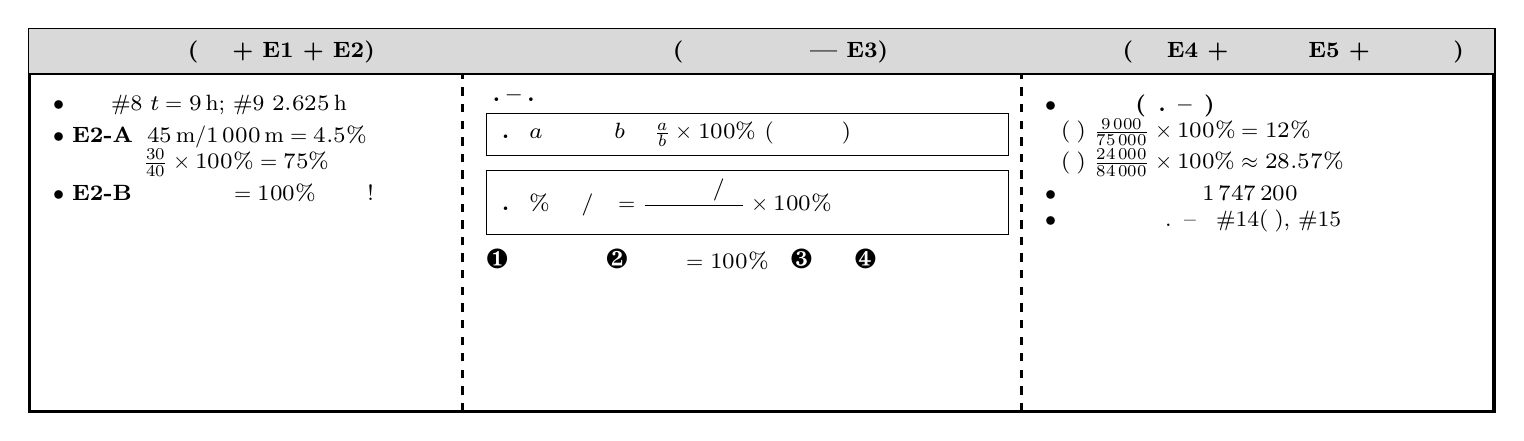
\begin{tikzpicture}[x=1cm, y=1cm, every node/.style={font=\footnotesize, text=black}]
  \draw[black, line width=1.2pt] (0,0) rectangle (18.6,4.85);
  \fill[headgray] (0,4.28) rectangle (18.6,4.85);
  \draw[black, line width=0.8pt] (0,4.28) -- (18.6,4.28);
  \draw[black, line width=0.85pt, dashed] (5.5,0) -- (5.5,4.28);
  \draw[black, line width=0.85pt, dashed] (12.6,0) -- (12.6,4.28);

  \node at (2.75,4.56) {\textbf{ផ្នែកឆ្វេង (កំណែ + \en{E1} + \en{E2})}};
  \node at (9.05,4.56) {\textbf{ផ្នែកកណ្ដាល (ខ្លឹមសារគោលរក្សាទុក — \en{E3})}};
  \node at (15.6,4.56) {\textbf{ផ្នែកស្ដាំ (គំរូ \en{E4} + ប្រតិបត្តិ \en{E5} + កិច្ចការផ្ទះ)}};

  \node[anchor=north west, align=left] at (0.18,4.14) {
    $\bullet$ \textbf{កំណែ៖} \#8 $t=9\unit{h}$; \#9 $2.625\unit{h}$\\[2pt]
    $\bullet$ \textbf{\en{E2-A}៖} $45\unit{m}/1\,000\unit{m} = 4.5\%$\\
    \hspace*{0.25cm}សិស្សជាប់៖ $\frac{30}{40}\times 100\% = 75\%$\\[2pt]
    $\bullet$ \textbf{\en{E2-B}៖} ប្រាក់ថ្លៃដើម $= 100\%$ ជានិច្ច!
  };

  \node[anchor=north west, align=left] at (5.68,4.14) {
    {\muol\fontsize{8.2pt}{12pt}\selectfont ២\enbf{.}១\enbf{--}២\enbf{.}២ ភាគរយ ប្រាក់ចំណេញនិងប្រាក់ខាត}\\[3pt]
    \fbox{\parbox{6.4cm}{\textbf{២.១៖} $a$ ជាភាគរយនៃ $b$ គឺ $\frac{a}{b}\times 100\%$ (ឯកតាដូចគ្នា)}}\\[4pt]
    \fbox{\parbox{6.4cm}{\textbf{២.២៖} $\% \text{ចំណេញ/ខាត} = \dfrac{\text{ប្រាក់ចំណេញ/ខាត}}{\text{ប្រាក់ថ្លៃដើម}}\times 100\%$}}\\[4pt]
    \cnum{1} ឯកតាដូចគ្នា \; \cnum{2} ថ្លៃដើម $=100\%$ \; \cnum{3} ដក \; \cnum{4} ថ្លៃលក់
  };

  \node[anchor=north west, align=left] at (12.78,4.14) {
    $\bullet$ \textbf{គំរូរថយន្ត (ទំ.៣២--៣៣)៖}\\
    \hspace*{0.2cm}(ក) $\frac{9\,000}{75\,000}\times 100\% = 12\%$\\
    \hspace*{0.2cm}(ខ) $\frac{24\,000}{84\,000}\times 100\% \approx 28.57\%$\\[2pt]
    $\bullet$ \textbf{ប្រតិបត្តិម៉ូតូពូសុខ៖} $1\,747\,200\riel$\\
    $\bullet$ \textbf{កិច្ចការផ្ទះ៖} ទំ.៤១--៤២ \#14(ក), \#15
  };
\end{tikzpicture}
\end{center}

\secstrip{២. ចម្លើយផ្ទៀងផ្ទាត់រហ័សសម្រាប់សន្លឹកកិច្ចការសិស្ស (ទំព័រ ១ និង ទំព័រ ២)}{\en{Answer Key}}

\begin{tcolorbox}[
  enhanced, sharp corners, colback=white, colframe=black,
  boxrule=0.8pt, boxsep=1.5pt, top=3pt, bottom=3pt, left=5pt, right=5pt,
  after skip=3.5pt
]
  \fontsize{8.8pt}{13.2pt}\selectfont
  $\bullet$ \textbf{ផ្នែក \en{E1}៖} \textbf{សិស្ស ខ ($25\%$)} ត្រឹមត្រូវ; ត្រូវធៀបនឹង\textbf{ប្រាក់ថ្លៃដើម} ។\\[2pt]
  $\bullet$ \textbf{ផ្នែក \en{E2}៖} \textbf{សកម្មភាព ១៖} $1\unit{km} = \mathbf{1\,000}\unit{m} \implies \mathbf{4.5\%}$; តេស្តសិស្សជាប់ $\mathbf{75\%}$ ។ \textbf{សកម្មភាព ២៖} ចំណេញ $=$ ថ្លៃលក់ $-$ \textbf{ប្រាក់ថ្លៃដើម}; ខាត $=$ \textbf{ប្រាក់ថ្លៃដើម} $-$ ថ្លៃលក់; គូសរង្វង់ \textbf{ប្រាក់ថ្លៃដើម} ទាំងពីរករណី ។\\[2pt]
  $\bullet$ \textbf{ផ្នែក \en{E4}៖} (ក) ដើម $75\,000\usd$, ចំណេញ $9\,000\usd \implies \mathbf{12\%}$; (ខ) ដើមលោកលីស្រ៊ុន $84\,000\usd$, ខាត $24\,000\usd \implies \mathbf{28.57\%}$ ។\\[2pt]
  $\bullet$ \textbf{ផ្នែក \en{E5}៖} \textbf{១) ប្រតិបត្តិ ១៖} $\mathbf{95\%}$, $\mathbf{92\%}$; $2\unit{kg}=2\,000\unit{g} \implies \mathbf{17.5\%}$ ។ \textbf{២) ម៉ូតូពូសុខ៖} ខាត $492\,800\riel \implies$ ថ្លៃលក់ $\mathbf{1\,747\,200\riel}$; បិទ \en{E1} $\mathbf{25\%}$ ។ \textbf{៣) វិនិច្ឆ័យ \en{A--D}៖} ជម្រើស \textbf{\en{B}} ។ \textbf{៤) សំបុត្រចេញ៖} (ក) $\mathbf{12.5\%}$; (ខ) $\mathbf{15\%}$ ។
\end{tcolorbox}

\secstrip{៣. ចម្លើយលម្អិតនៃកិច្ចការផ្ទះ (សម្រាប់ផ្ទៀងនៅដើមម៉ោងបន្ទាប់ ២.៣--២.៤)}{សៀវភៅគោល ទំ.៤១--៤២}

\begin{tcolorbox}[
  enhanced, sharp corners, colback=white, colframe=black,
  boxrule=0.8pt, boxsep=1.5pt, top=3pt, bottom=3pt, left=5pt, right=5pt
]
  \fontsize{8.6pt}{12.8pt}\selectfont
  $\bullet$ \textbf{\#14 ក (ទំ.៤១--៤២)៖} ភាគរយសៀវភៅមិនមែនប្រលោមលោក $= 100\% - 28\% = 72\%$ ។ ផលសងភាគរយ $= 72\% - 28\% = 44\%$ ត្រូវនឹង $1\,980$ ក្បាល $\implies$ ចំនួនសៀវភៅសរុប $= \dfrac{1\,980 \times 100}{44} = \mathbf{4\,500\text{ ក្បាល}}$ ។ សៀវភៅប្រលោមលោក $= 28\% \times 4\,500 = \mathbf{1\,260\text{ ក្បាល}}$ និងមិនមែនប្រលោមលោក $= 1\,260 + 1\,980 = \mathbf{3\,240\text{ ក្បាល}}$ ។\\[3pt]
  $\bullet$ \textbf{\#15 (ទំ.៤២)៖} ចំណាយ $20\%$ នៃ $250\,000\usd = 50\,000\usd \implies$ ប្រាក់សល់ $= 200\,000\usd$ ។ ប្រាក់គ្រប់គ្រងរបស់លោកសុង $= 16\% \times 200\,000\usd = 32\,000\usd \implies$ ប្រាក់សល់ចែកតាមដើមទុន $= 200\,000 - 32\,000 = 168\,000\usd$ ។ ផលធៀបដើមទុន $= 800\,000 : 900\,000 : 1\,100\,000 = 8 : 9 : 11$ (សរុប $28$ ចំណែក, $1$ ចំណែក $= \frac{168\,000}{28} = 6\,000\usd$)៖ លោកសុងទទួលសរុប $32\,000 + 8(6\,000) = \mathbf{80\,000\usd}$, លោកចេនទទួល $9(6\,000) = \mathbf{54\,000\usd}$, និងលោកស្រីភីទទួល $11(6\,000) = \mathbf{66\,000\usd}$ ។
\end{tcolorbox}

\end{document}
